%% Preambel
\documentclass[conference,compsoc,final,a4paper]{IEEEtran}
\usepackage[utf8]{inputenx}

%% Bitte legen Sie hier den Titel und den Autor der Arbeit fest
\newcommand{\autoren}[0]{Mueller, Thorsten}
\newcommand{\dokumententitel}[0]{Overcoming the barriers of newcomers to software crowdsourcing by understanding their motivations and barriers}

% Pakete einbinden, die benötigt werden
\usepackage{scrpage2}
\usepackage{graphicx}             % Bilder einbinden
\usepackage{xcolor}               % Color support
\usepackage{amsmath}              % Matheamtische Formeln
\usepackage{amsfonts}             % Mathematische Zeichensätze
\usepackage{amssymb}              % Mathematische Symbole
\usepackage{float}                % Fließende Objekte (Tabellen, Grafiken etc.)
\usepackage{booktabs}             % Korrekter Tabellensatz
\usepackage[printonlyused]{acronym}  % Abkürzungsverzeichnis [nur verwendete Abkürzugen]
\usepackage{makeidx}              % Sachregister
\usepackage{listings}             % Source Code listings
\usepackage{listingsutf8}         % Listings in UTF8
\usepackage[hang,font={sf,footnotesize},labelfont={footnotesize,bf}]{caption} % Beschriftungen
\usepackage[scaled]{helvet}       % Schrift Helvetia laden
\usepackage[sf,bf,small]{titlesec} % Einstellungen für Überschriften
\usepackage[absolute]{textpos}	  % Absolute Textpositionen (für Deckblatt)
\usepackage{calc}                 % Berechnung von Positionen
\usepackage{blindtext}            % Blindtexte
\usepackage[bottom=40mm,left=35mm,right=35mm,top=30mm]{geometry} % Ränder ändern
\usepackage{setspace}             % Abstände korrigieren
\usepackage{ifthen}               % Logische Bedingungen mit ifthenelse
\usepackage{scrhack}              % Get rid of tocbasic warnings
%\usepackage[pagebackref=false]{hyperref}  % Hyperlinks
%\usepackage{rotating}             % Seiten drehen

%\setlength{\bibitemsep}{1em}     % Abstand zwischen den Literaturangaben
%\setlength{\bibhang}{2em}        % Einzug nach jeweils erster Zeile

% Farben definieren
\definecolor{linkblue}{RGB}{0, 0, 100}
\definecolor{linkblack}{RGB}{0, 0, 0}
\definecolor{comment}{RGB}{63, 127, 95}
\definecolor{darkgreen}{RGB}{14, 144, 102}
\definecolor{darkblue}{RGB}{0,0,168}
\definecolor{darkred}{RGB}{128,0,0}
\definecolor{javadoccomment}{RGB}{0,0,240}

% Einstellungen für das Hyperlink-Paket
\hypersetup{
    colorlinks=true,      % Farbige links verwenden       
%    allcolors=linkblue,
    linktoc=all,          % Links im Inhaltsverzeichnis
    linkcolor=linkblack,  % Querverweise
    citecolor=linkblack,  % Literaturangaben
	filecolor=linkblack,  % Dateilinks
	urlcolor=linkblack    % URLs
}

% Einstellungen für Quelltexte
\lstset{     
      xleftmargin=0.2cm,     
      basicstyle=\footnotesize\ttfamily,
      keywordstyle=\color{darkgreen},
      identifierstyle=\color{darkblue},
      commentstyle=\color{comment}, 
      stringstyle=\color{darkred}, 
      tabsize=2,
      lineskip={2pt},
      columns=flexible,
      inputencoding=utf8,
      captionpos=b,
      breakautoindent=true,
	  breakindent=2em,
	  breaklines=true,
	  prebreak=,
	  postbreak=,
      numbers=none,
      numberstyle=\tiny,
      showspaces=false,      % Keine Leerzeichensymbole
      showtabs=false,        % Keine Tabsymbole
      showstringspaces=false,% Leerzeichen in Strings
      morecomment=[s][\color{javadoccomment}]{/**}{*/},
      literate={Ö}{{\"O}}1 {Ä}{{\"A}}1 {Ü}{{\"U}}1 {ß}{{\ss}}2 {ü}{{\"u}}1 {ä}{{\"a}}1 {ö}{{\"o}}1
}

\urlstyle{same}

\titlespacing{\paragraph}{0pt}{1ex}{2.0ex}
\titlespacing{\subsubsection}{0pt}{3ex}{0.0ex}
\titlespacing{\subsection}{0pt}{4ex}{0.2ex}
\titlespacing{\section}{0pt}{7ex}{1ex}
\titleformat*{\subsubsection}{\sffamily\itshape\bfseries\small}
\titleformat*{\paragraph}{\sffamily\bfseries\small}


% Einstellungen für Überschriften
\renewcommand*{\chapterformat}{%
  \Large\chapapp~\thechapter   % Große Schrift
  \vspace{0.3cm}               % Abstand zum Titel des Kapitels
}

% Abstände für die Überschriften setzen

% In der Kopfzeile nur die kurze Kapitelbezeichnung (ohne Kapitel davor)
\renewcommand*\chaptermarkformat{\thechapter\autodot\enskip}
\automark[chapter]{chapter}

% Einstellungen für Schriftarten
\setkomafont{pagehead}{\normalfont\sffamily}
\setkomafont{pagenumber}{\normalfont\sffamily}
\setkomafont{paragraph}{\sffamily\bfseries\small}
\setkomafont{subsubsection}{\sffamily\itshape\bfseries\small}
\addtokomafont{footnote}{\footnotesize}
\setkomafont{chapter}{\LARGE\selectfont\bfseries}

% Wichtige Abstände
\setlength{\parskip}{0.2cm}  % 2mm Abstand zwischen zwei Absätzen
\setlength{\parindent}{0mm}  % Absätze nicht einziehen
\clubpenalty = 10000         % Keine "Schusterjungen"
\widowpenalty = 10000        % Keine "Hurenkinder"
\displaywidowpenalty = 10000 % Keine "Hurenkinder"
\renewcommand{\footnotesize}{\fontsize{9}{10}\selectfont} % Größe der Fußnoten
\setlength{\footnotesep}{8pt} % Abstand zwischen den Fußnoten

% Index erzeugen
\makeindex

% Einfacher Font-Wechsel über dieses Makro
\newcommand{\changefont}[3]{
\fontfamily{#1} \fontseries{#2} \fontshape{#3} \selectfont}

% Eigenes Makro für Bilder
\newcommand{\bild}[3]{
\begin{figure}[h]
  \centering
  \includegraphics[width=#2]{#1}
  \caption{#3}
  \label{#1}
\end{figure}}

% Wo liegt Sourcecode?
\newcommand{\srcloc}{src/}

% Wo sind die Bilder?
\graphicspath{{bilder/}}

% Makros für typographisch korrekte Abkürzungen
\newcommand{\zb}[0]{z.\,B.\ }
\newcommand{\dahe}[0]{d.\,h.\ }
\newcommand{\ua}[0]{u.\,a.\ }

% Flags für Veröffentlichung und Sperrvermerk
\newboolean{hsmapublizieren}
\newboolean{hsmasperrvermerk}
 % Weitere Einstellungen aus einer anderen Datei lesen

% Eigentliches Dokument beginnt hier
% ----------------------------------------------------------------------------------------------------------

% Kurze Zusammenfassung des Dokuments
\begin{abstract}
% a quick summary or overview of the entire paper 
Outsourcing work is a well known by companies. Software crowdsourcing has a lot of potential to become a major technology in software development, as it already has a huge rise over the last years. To provide a deeper understanding of software crowdsourcing, this paper will explain the different types of crowdsourcing and also how software crowdsourcing works. The aim of this systematic literature review is to clearify the question: \textit{How newcomers can successfully work on software crowdsourcing projects?} To do so, the paper first provides motivations as well as barriers to newcomers and companies. With the knowledge of both, the motivations and barriers, it is easier to understand the barriers of newcommers and as a result how to overcome those. In addition, recommendations to overcome the barriers will be revealed. 
%OTCs nicht vergessen
\end{abstract}

\tableofcontents

% Abschnitte mit \section und Unterabschnitte mit \subsection
\section{Introduction}
\ac{SW CS} had a huge popularity rise in the last few years, even it exits for a very long time. For community projects, such as Linux or Firefox, it is a well known and existing dependant technique. Without the crowd such projects, e.g. elementary OS, Apache and many more would not be possible. With the rise of \ac{SW CS} many people try out crowdsourcing. Before somebody can successful contribute to an project there are several barriers, which specially newcomers have to overcome. For each crowdsourcing project it is important to reduce the barriers as much as possible. \ac{SW CS} and \ac{OSS} projects are existing because there is an interest in the crowd to contribute to a specific project. Without the interst of the crowd, the project will not find enough new contributors and as a result it will die \cite{Ref}. A problem with the barriers is, that every newcomer has their own mental model of crowdsourcing before they start to work on a project\cite{Ref}. Due to this individual mental model it is not completely possible to weight the barriers. Knowing this fact, this paper weights the barriers by the amount found in the secondary research. Moreover, to better understand and how to overcome the barriers, it is also important to know what drives software developers to start contributing to a \ac{SW CS} project. To receive a better and deeper understanding of the motivations and hurdles it is important to look also to similiar techniques beside \ac{SW CS}. Those technique are; \ac{FLOSS}, \ac{FOSS} and \ac{OSS}. Due to those techniques are all very similiar to \ac{SW CS}, all of them are included in the search for barriers newcomers are facing before they successful contribute in such an project. Also, those techniques are included in the research of motivations and how to overcome the barriers.\newline
The second section explains how the research took place. In the third section crowdsourcing is explained. By doing so, everybody has the same basis to discuss or provide feedback to the research topic. The fourth section reveals motivations for newcomers. Followed by the motivations, the barriers for newcomers are categorized and listed in the fith section. After the foundation on how to overcome barriers is set, recommondations to lower the barriers for companies and platforms are revealed. This section includes also, how software visualization tools can help to reduce barriers. The last section shows the result of this paper.

\section{Research Method}
To find relevant scientific papers i used the following search engines, 'GoogleScholar', 'IEEE Xplore', 'ACM Digital Library and 'Springer Link'. 
Due to \ac{SW CS} is a widely spreaded term, it was hard to do a systematic literature review. With the following search term, it had to be included in the title \textit{("Barriers" OR "Newcomers" OR Motivation") AND ("Software Crowdsourcing" OR "Open Source Software" OR "Free Libre Open Source Software")}, GoogleScholar showed 907 results and IEEEXplore showed 141 results. SpringerLink did not found any title regarding to the search query. Of the 141 results 14 papers were usefull for this secondary research. To not go through the 907 papers, keyword searches helped to find additional papers. To create this paper I used X researches. 

\section{State of the art}
\begin{figure}
	\center
	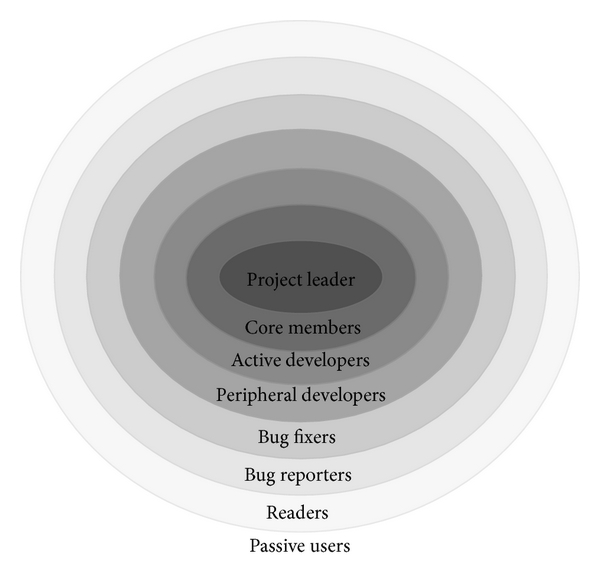
\includegraphics{General-structure-of-an-OSS-community-based-on-the-onion-model-described-in-4.png}
	\caption{Onion model of an OSS community \cite{Ye2003}}
	\label{img:onion_model}
\end{figure}

Nowadays crowdsourcing can be found in a lot of different areas as the system gets more an more popular. Due to the popularity of crowdsourcing it is no incident that you will find a variety of crowdsourcing platforms, e.g. Idea Bounty, CrowdSpring, 99Designs, TopCoder and many more. Due to the high use of the word it is not possible to coherently classify the term 'crowdsourcing'[1]. As Enrique Estellés-Arolas and Fernando González-Ladrón-de-Guevara in the article 'Towards an integrated crowdsourcing definition'\cite{Estelles-Arolas2012} wrote: 
\begin{quote}
The name crowdsourcing is formed from two words: crowd, making reference to the people who participate in the initiatives; and sourcing, which refers to a number of procurement practices aimed at finding, evaluating and engaging suppliers of goods and services.
\end{quote}

%The different models of Crowdsourcing (competetive vs collaborative)
\subsection{Crowdsourcing models}
During the literature review I found four different types of crowdsourcing models.
Within those four models there are two major ways of \ac{SW CS}. The competetive method, which had a incredible increase during the last years. The oldest method is the collaborative, which has its roots in the \ac{OSS} and is still a huge factor if or if not crowdsourced projects are successfull. \newline

Such project developed during the years their own model of the community, which is shown in figure \ref{img:onion_model}. At the centre there are the core developers. Those need to have a large technical expertise as well as good understanding of the project, because those are the project leaders and the core contributors. The project leaders control the evolution of the project, wheras the core contributors are also considering the project evolution are they the ones who provide the most source code to the project. In the next layers there are the co-developers (the active- and peripheral developers). They contribute often source-code and also have to be familiar with the project. Even more outside there are the active users (bug fixers and bug reporters). The active users provide bug search and report. Also, they help the community by answering questions. As a result of the interaction with the community, they bring in new feature ideas. The two outermost layers are the users of such a \ac{OSS} project. They use but without giving something in return \cite{Crowston2005, Wolff-Marting2013}.
It is important to get people motivated to contribute to such projects. Otherwise, those projects would collabse. In \ac{OSS} projects there are always motivations, that brings developers closer to the core. Also, there are forces which keep the developers away from the core \cite{Wolff-Marting2013}. \newline

The first model ist the competetive, also called commercial, model. In this model the collaborator are contestants to eachother\cite{LaToza2016, Riehle2007}. A natural motivation in this model is to compete against each other and the winner will get a reward of the company. With those two motivations it is no wonder that this model gained a lot of attention in software development. The most popular platform for this model is TopCoder (www.topcoder.com) with over one million people in the community and over seven thousand challanges per year. 
An old model is the 'Peer Production', it is also called to be the community version of SW CS \cite{LaToza2016, Riehle2007}.'Peer Production' is an \ac{OSS} procedure which consists of software projects where the community contributes to their favorite project. There is a huge amount of those community based \ac{OSS} projects nowdays. Some of the most known are Linux, Firefox, Apache and Atom. Those projects are great example how the crowd can create a great product. Also this model depents that a lot of people contribute to the project. Like the onion model of \ac{FLOSS} projects the onion model for this crowdsourcing would look similiar. At the core there would be the innovation leaders, those who lead the project. Around them there would be the key contributors, those contributors who work constanly on the project. Those contributors who are just active sometimes, e.g. to fix bugs, are at the outside of the onion model.
Another model is called 'Microtasking'\cite{LaToza2016}. In this model the tasks will split up to several small task. With this procedure there will be a lot of small tasks. Without much time needed to complete one task, many contributors are up to do the task. With this redundancy there will be also some differencies in the solutions. Due to those solutions the requester can select the for him best suited solution. 
A similiar to the previous model is the 'Economic model'\cite{Tsai2014}. The goal of this model is also to maximize the contributions.
The companies are creating strategies to include the crowd. Also, the winner, sometimes also the best three solutions, will receive a reward for his contribution.

%Level 1-4
\subsection{Levels of Crowdsourcing}
The ideas of this subsection were received by the article 'Cloud-based Software Crowdsourcing (Dagstuhl Seminar 13362)'\cite{Huhns2013} written by Huns et al. Due to it was the only paper which described the different levels of crowdsourcing, the ideas will be from this article.\newline
As well there are different method of crowdsourcing there are also different level's. Those levels describe how many contributors work on the contribution as well as how large the task is and how much time the contributors have. Those level's are called 'Level 1' up to 'Level 4', where the first level is describes the individual developer. In this level the commiters have clear tasks, which they have to solve within a few moths. Also, the individuals developers as well as the projects can be ranked.
The second level uses small teams with up to ten people per team. Those teams have up to one year time, depending on the project, to develop their solution for the given task. Also it allows that the developers will get feedback and thoughts from the stakeholders and the community during the developing process. 
The next larger level has teams of more than 10 and up to 100 people and a development time of up to two years. Due to this large time span and the larger teams the crowdsourcing platforms for 'Level 3' crowdsourcing need to have an automated cross-verification and is not suited for commercial crowdsourcing, as well as the largest level. With this technique the platform will automatically check if the requirements are met or not.
The largest level has international factors. The developers, from several countries, develop a large and flexible system. Due to the international factors, those projects has to overcome additional barriers before they can succeed. Those barriers are social-cultural barriers, which will be explained in Section X.



\section{Motivation for software crowdsourcing}
As humans we have two types of motivation. One is the 'intrinsic motivation' and the other one is the 'extrinsic motivation'. Intrinsic Motivation describes the motivation of doing a task for inborn satisfaction\cite{Ryan2000}. Regarding to \ac{SW CS} this could be to contribute with reasons like; fun and enjoyment, technical learning, altruism. The oponent of the intrinsic motivation is the extrinsic motivation. Extrinsic motivation play always a role, if the person gets something afterwards to do the task \cite{Ryan2000}.Examples therefor are the career status, reputation, fame, community identification. All of the motivations showed in this section can be defined as instrinsic or extrinsic motivation. Also, in the table \ref{tbl:CntribMoti} you will see that there a slightly more intrinsic motivations than extrinsic motivations from a contributors view. As the subsection "Contributer Perspectives" shows, the amount of both motivation types is similiar. This similiarity is important, because to much of one motivation type can have negative effects on the other type \cite{Hossain2012a}. From a stakeholder views there are only extrinsic goals, as shown in table \ref{tbl:StkhldrMoti}. For companies the similarity of both motivatinos does not count, because the main goal of a company is to get something in return for their work.

%companies
\subsection{Stakeholder Perspectives}
The perspectives for the stakeholders were found in the following papers;
\begin{itemize}
	\item Riehle; The Economic Motivation of Open Source Software: Stakeholder Perspectives\cite{Riehle2007}
	\item LaToza and van der Hoek; Crowdsourcing in Software Engineering: Models, Motivations, and Challenges\cite{LaToza2016}
	\item Hossain; Crowdsourcing: Activities, incentives and users' motivations to participate\cite{Hossain2012}
	\item Tsai et al.; Cloud-Based Software Crowdsourcing\cite{Tsai2014}
\end{itemize}
As a stakeholder views, there are in depth reasons why you should consider investing in the \ac{OSS} market. The companies, which are using the \ac{OSS} market, do not sell the product. More likely, they sell the provision, maintenance and the support for the product. Another motivation is; the companies consider more the opinions of the crowd and let them choose the task to work so. By doing so, more people of the crowd will contribute and also they will find more qualitive solutions to their task. Due to the last two points, the customers will trust your company and the product more. With this in the knowledge the company will have less marketing costs. Also, the number of customers will increase rapidly. The companies can hire and fire employees more easily, because there is an large pool of people who fit to the companie or did already worked on the project. Moreover, it is easier to find and employ specialists, due to every project has its 'core worker'. Those core worker are worker, who are specialists in the projects and also work a long time on it. So the core worker have a lot of knowledge and it is also shown that they lead innovations in the projects\cite{Hossain2012, XY}. As a result of finding an employing specialists those specialists can develop more innovative products. With the diversity of the crowd, companies will get alternative solutions. When a company start to enter the \ac{OSS} field, they will have less time until the next innovative idea comes up. Also, they will have variable costs. It will be easier to share information and they will find an increase in the development speed. The increase in the development speed is found due to the crowd, as they overtake parts of the development. By spending a longer time on the \ac{OSS} market, your customers will become more loyal and the companies will find less risks by launching a new product. Also, the companies will have a increase of the quality of their software. This is a result of the trust by the customers that the company provises, maintain and support their product for a longer time. All those motivations are listed in the table \ref{tbl:StkhldrMoti}.


\begin{table*}
\centering
\caption{Stakeholder motivations to use software crowdsourcing}
\renewcommand{\arraystretch}{1.5}
	\begin{tabular}{lrrr} %p{4.5cm}p{1cm}p{1cm}p{1cm} - 
		\textbf{Motivation} & \textbf{Motivation type} & \textbf{Found X times} & \textbf{Papers} \\
		
		\multicolumn{4}{l}{\textbf{Extrinsic Motivation}} \\
		
		the company will have less marketing costs & Extrinsic & 2 & \cite{Hossain2012, Tsai2014}\\

		it is easier to find and employ specialists & Extrinsic & 2 & \cite{LaToza2016, Tsai2014}\\
		
		specialists can develop more innovative products & Extrinsic & 2 & \cite{Hossain2012, Tsai2014} \\
		
		companies will get alternative solutions & Extrinsic & 2 & \cite{LaToza2016, Tsai2014}\\
		
		the company sell the provision, maintenance and the support for the product & Extrinsic & 1 & \cite{Riehle2007} \\
		
		the company find more qualitive solutions to their task & Extrinsic & 1 & \cite{LaToza2016}\\
		
		the number of customers will increase rapidly & Extrinsic & 1 & \cite{Hossain2012} \\
		
		the companies can hire and fire employees more easily & Extrinsic & 1 & \cite{Riehle2007} \\
		
		the company will have less time until the next innovative idea comes up & Extrinsic & 1 & \cite{Hossain2012}\\
		
		the company will have variable costs & Extrinsic & 1 & \cite{LaToza2016}\\
		
		the customers will become more loyal & Extrinsic & 1 & \cite{Hossain2012} \\
		
		the companies will find less risks by launching a new product & Extrinsic & 1 & \cite{Hossain2012}\\
		
		the companies will have a increase of the quality of their software & Extrinsic & X & XY
		
		

	\end{tabular}
	\label{tbl:StkhldrMoti}
\end{table*}


%contributors
\subsection{Contributor Perspectives}
The motivations for this subsection were found in the following papers;
\begin{itemize}
	\item Hannebauer et al.; An Exploratory Study of Contribution Barriers Experienced by Newcomers to Open Source Software Projects\cite{Hannebauer2014}
	\item Hannebauer and Gruhn; On the Relationship Between Newcomer Motivations and Contribution Barriers in Open Source Projects\cite{Hannebauer2017}
	\item Lee et al.; Understanding the Impressions, Motivations, and Barriers of One Time Code Contributors to FLOSS Projects: A Survey\cite{Lee2017}
	\item LaToza and van der Hoek; Crowdsourcing in Software Engineering: Models, Motivations, and Challenges\cite{LaToza2016}
	\item Hossain; Users' motivation to participate in online crowdsourcing platforms\cite{Hossain2012a}
\end{itemize}
A more detailed view and who wrote about which paper will be shown in figure XY.\newline
The motivations for the contributors were listed in several papers. The most named motivation is; improvement of programming skills or learn a new technology. I combined those two motivations because the goal of both is to improve yourself, no matter it is by increasing the developing skills or by learning a complete new developing language. Close to this motivation is that contributors want to learn about the project technologies. The second most motivation I found, is the reason that the contributors need a modification for their own project. Similiar to this motivation I found also that a motivation is to make the project interoperable with one's own products. As often as the motivation before, contributors mentioned also that they enjoy programming. Similar to the contributors enjoy programming there are also contributors who enjoy the intellecutal challenge. Some contributors mentioned also that they want to give something back to the community. Close to the last motivation, to consult to \ac{FLOSS} projects was also found. The belief in the idea of \ac{OSS} projects were also named as motivation. Also evaluating a project was found as a motivation to contribute and to give feedback to the project community. Try out \ac{OSS} software projects and to join a community was also mentioned as motivation. By submitting patches, satisfaction will derive from working in a project and with the community. Also, that the changes will be reviewed by others is also a motivation to contribute. A missing feature is also called to be a motivation. To gain the respect of the community was found bei Hannebauer. Personal visibility and similiar to it reputation were also revelead to motivate contributors. Some contributors maybe get paid to contribute, others may get a reward by submitting. The last motivation I could find is that the contributors will have only to contribute once. They will not have to rebuild their patch for the next version of the project again. As well as the stakeholder motivations, those motivations will be divded into intrinsic and extrinsic motivation and listet in table \ref{tbl:CntribMoti}. With this table you will get a good overview of the contributor motivations.

\begin{table*}
\centering
\caption{Motivations to contribute to a software crowdsourcing project}
\renewcommand{\arraystretch}{1.5} %die Zeilenabstände um 50% vergrößern
	\begin{tabular}{lrrr} %p{4.5cm}p{1cm}p{1cm}p{1cm} - 
		\textbf{Motivation} & \textbf{Motivation type} & \textbf{Found X times} & \textbf{Papers} \\
		
		\multicolumn{4}{l}{\textbf{Intrinsic Motivation}} \\
		
		improvement of programming skills or learn a new technology & Intrinsic & 4 & \cite{Hannebauer2014,Hannebauer2017,Lee2017,LaToza2016} \\
		
		enjoy programming & Intrinsic & 3 & \cite{Hannebauer2017, Hossain2012a, LaToza2016} \\
		
		want to give something back to the community & Intrinsic & 3 & \cite{Hannebauer2014, Hossain2012a, LaToza2016} \\
		
		want to learn about project technologies & Intrinsic & 1 & \cite{Hannebauer2014} \\
		
		enjoy the intellectual challenge & Intrinsic & 1 & \cite{Hannebauer2014} \\
		
		to consult FLOSS projects & Intrinsic & 1 & \cite{Hannebauer2014} \\
		
		The belief in the idea of open source projects & Intrinsic & 1 & \cite{Hannebauer2017} \\
		
		evaluating a project & Intrinsic & 1 & \cite{Hannebauer2014} \\
		
		try out open source software projects & Intrinsic & 1 & \cite{Hannebauer2017} \\
		
		to join a community & Intrinsic & 1 & \cite{Hannebauer2017} \\
		
		satisfaction will derive from working in a project and with the community & Intrinsic & 1 & \cite{Hannebauer2014} \\
		
		the contributors will have only to contribute once & Intrinsic & 1 & \cite{xy}\\
		
		
		\multicolumn{4}{l}{\textbf{Extrinsic Motivation}} \\
		
		need a modification for their own project & Extrinsic & 3 & \cite{Hannebauer2014,Hannebauer2017,Lee2017} \\
				
		personal visibility and reputation & Extrinsic & 2 & \cite{Hannebauer2014, Hossain2012a} \\		
		
		make the project interoperable with one's own products & Extrinsic & 1 & \cite{Hannebauer2014} \\
		
		the changes will be reviewed by others & Extrinsic & 1 & \cite{Hannebauer2014} \\
		
		gain respect of the community & Extrinsic & 1 & \cite{Hannebauer2014} \\
		
		get a reward or paid to contribute & Extrinsic & 1 & \cite{Lee2017} \\
	\end{tabular}
	\label{tbl:CntribMoti}
\end{table*}









\section{barriers faced by newcomers}
For this section I used 13 researches. To not overload the the text with citates, I choosed to cite the first view barriers. With those hurdles I will create a reference to all researches I used, to find barriers, in my systematic literature review.\newline
There are many barriers newcomers face by contributing for the first time. Some barriers are larger and other are smaller. I found in my literature review 71 barriers, why newcomer may not contribute to an crowdsourcing project or become a one time contributor. I conducted barriers, which have semantically the same meaning. Also, I subdivided the barriers into six main categories, as you can see in figure\ref{img:hurdles_categories}. Some of the categories will be further subdivided to get a better overview. This categorization and conducting the barriers will provide a more simplified and a more meaningfull statement. 
The barriers of the categories, which will not be further divided, will be presented in tables. Otherwise the figure to present the barriers would take too much space of the paper.

\begin{figure*}
	\center
	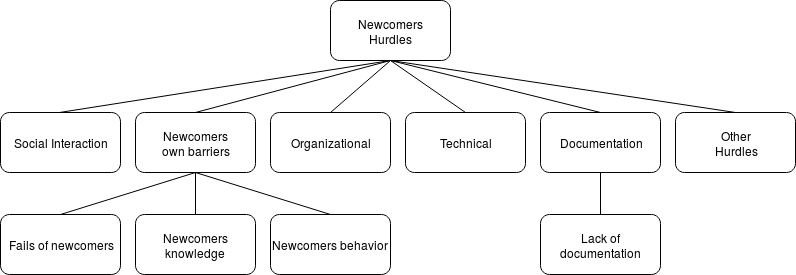
\includegraphics[scale=0.65]{BarriersCategorized.png}
	\caption{Categories of newcomers hurdles}
	\label{img:hurdles_categories}
\end{figure*}


\subsection{Organizational}
The barriers presented in this subsection are avoidable. Anyway, the barriers are created by the stakeholders as well as by the contributors. The hurdles in this section are always painfull, specially because it is easy to get loose of them.\newline
The hardest barrier I found is to submit the created solution. This hurdle is mainly a result of the documentation which the stakeholders have. As the lack of documentation was overall the second most reason I found in my research. Also, to obtain a current version of the source code was mentioned to be a problem in some projects. Similiar to it, inadequate procedures were also mentioned by newcomers as a reason to stop working on the project.

\begin{table}
\centering
\caption{Organizational barriers}
\renewcommand{\arraystretch}{1.5} %die Zeilenabstände um 50% vergrößern
	\begin{tabularx}{\linewidth}{Xrr} 
		\textbf{Barrier} & \textbf{Found X times} & \textbf{Papers} \\
		
		\multicolumn{3}{l}{\textbf{Organizational Barriers}} \\
		
		submitting their solution & 5 & \cite{Hannebauer2014,Hannebauer2017,Lee2017,Steinmacher2015c,Steinmacher2014a} \\
		
		obtain the current version of the source code & 2 & \cite{Hannebauer2014,Hannebauer2017} \\
		
		inadquate procedures & 2 & \cite{Zanatta2017,Hannebauer2017} \\
		
		poor task management & 1 & \cite{Zanatta2017} \\
		
		an overload of information & 1 & \cite{Zanatta2017} \\
		
		the issues are not up to date & 1 & \cite{Steinmacher2015c} \\
		
		bureaucracy & 1 & \cite{Hannebauer2017} \\
		
	\end{tabularx}
	\label{tbl:Organizational_Barriers}
\end{table}

\subsection{Social Interaction}
Social interactions in forums or in mailing lists is a huge barrier, where newcomers have to jump over it. The hardest hurdle is that newcomers receive impolite answers and sometimes those included even frightening terms. Close to this barrier, newcomers also reported that they received delayed answers or they did not receive an answer at all. Some answers to newcomers did include too much advanced knowledge. Also, the newcomers sometimes did not receive feedback on their solution. Sometimes this feedback did come delayed, which may brought newcomers to stop further working on the project. Moreover,  newcomers want to contact a real person, as a lot of them are searching for a mentor. This might be a result of a language barrier for some newcomers as well as of problems with the community, which newcomers reported. Other newcomers may do not want this much support but they want the support on how to start with the project. All these hurdles are listet in the table \ref{tbl:Social_Barriers}.

\begin{table}
\centering
\caption{Social Interaction barriers}
\renewcommand{\arraystretch}{1.5} %die Zeilenabstände um 50% vergrößern
	\begin{tabularx}{\linewidth}{Xrr} 
		\textbf{Barrier} & \textbf{Found X times} & \textbf{Papers} \\
		
		\multicolumn{3}{l}{\textbf{Social Interaction Barriers}} \\		
		
		receiving impolite answers & 5 & \cite{Steinmacher2014b, Steinmacher2013, Steinmacher2014a, Steinmacher2015a, Steinmacher2014} \\
		
		finding a mentor & 4 & \cite{Steinmacher2014b, Steinmacher2014a, Steinmacher2015a, Steinmacher2014} \\
		
		receive delayed responses or no answer at all & 4 & \cite{Steinmacher2014b, Steinmacher2014a, Steinmacher2015a, Steinmacher2014} \\
		
		language barrier & 2 & \cite{Zanatta2017, Steinmacher2014a} \\
		
		problems regarding to the community & 2 & \cite{Hannebauer2017, Steinmacher2014} \\
		
		receiving a delayed feedback on the submitted work & 2 & \cite{Machado2017, Steinmacher2014a}\\
		
		newcomers have the need to contact and see their stakeholders in real & 2 & \cite{Steinmacher2015a, Steinmacher2014a}\\
		
		not receiving feedback on the submitted work & 1 & \cite{Machado2017} \\
		
		newcomers felt they did not get the support to start & 1 & \cite{Steinmacher2013} \\
		
		answers did include too advanced details & 1 & \cite{Steinmacher2014a} \\
			
	\end{tabularx}
	\label{tbl:Social_Barriers}
\end{table}

\subsection{Documentation Problems}
Here I will present all barriers regarding to documentation. Some of them will be more general and other are more specific. I splitted both kinds in the table XY.
Overall, a lack of documentation was the second most barrier which I could find. This displays how most of the of the companies work. They want a fast solution but then there is no time for the documentation. This common procedure makes it very hard to inpossible to start working on the project for newcomers. Also spread, unclear or even outdated documentation were named by problems regarding to the documentation. Also, tutorials were incomplete and outdated sometimes. On the other side a information overload due to the documentation was also mentioned as a barrier. The following more detailed problems with the documentation with figured out by the papers 'The Hard Life of Open Source Software Project Newcomers'\cite{Steinmacher2014b} and Preliminary Empirical Identification of Barriers Faced by Newcomers to Open Source Software Projects\cite{Steinmacher2014a}. The following hurdles provide a more insight view where the newcomers had more or less problems with the documentation. A lack of documentation on how to set up the workspace and about the project structure were the most named barriers. Those are very important, because the first should provide help, that the newcomer can work on the project and the other one should provide help that the contributors are able to understand the project. Another important barrier, which strengthens that the newcommers have a hard time to submit the solution, is the lack of documentation of the contribution process. Other barriers are a lack of design documents, a lack of code comments and a lack of the code documentation.

\begin{table}
\centering
\caption{Documentation barriers}
\renewcommand{\arraystretch}{1.5} %die Zeilenabstände um 50% vergrößern
	\begin{tabularx}{\linewidth}{Xrr} 
		\textbf{Barrier} & \textbf{Found X times} & \textbf{Papers} \\
		
		\multicolumn{3}{l}{\textbf{Documentation Barriers}} \\		
		
		lack of documentation & 7 & \cite{Zanatta2017, Hannebauer2017, Machado2017, Steinmacher2014b, Steinmacher2015c, Steinmacher2014a, Steinmacher2015a} \\
		
		outdated documentation & 4 & \cite{Steinmacher2014b, Steinmacher2014a, Steinmacher2015a, Steinmacher2014} \\
		
		an information overload & 3 & \cite{Steinmacher2014a, Steinmacher2015a, Steinmacher2014} \\
		
		incomplete or outdated tutorials & 2 & \cite{Steinmacher2015c, Steinmacher2014a} \\
		
		unclear documentation & 2 & \cite{Steinmacher2014b, Steinmacher2014a} \\
		
		spread documentation & 2 & \cite{Steinmacher2014b, Steinmacher2014a}\\
		
		problems related to the task documentation & 1 & \cite{Zanatta2017}\\
		
		\multicolumn{3}{l}{\textbf{Details of the documentation barriers}} \\	
		
		lack of documentation on how to set up the workspace & 2 & \cite{Steinmacher2014b, Steinmacher2014a} \\
		
		lack of documentation on the project structure & 2 & \cite{Steinmacher2014b, Steinmacher2014a} \\
		
		lack of documentation about the process documentation & 1 & \cite{Steinmacher2014b} \\
		
		lack of design documents & 1 & \cite{Steinmacher2014a} \\
		
		lack of code comments & 1 & \cite{Steinmacher2014a} \\
				
		lack of code documentation & 1 & \cite{Steinmacher2014a} \\
			
	\end{tabularx}
	\label{tbl:Documentation_Barriers}
\end{table}

\subsection{Technical hurdles}
This subsection had by far the most issues, with 17 barriers. Also, it includes the biggest barrier for newcomers. This one is to rebuild the system. The lack of documentation about how to set up the workspace from the section before strengthen this hurdle. This barrier can be extended, because platofrm and library dependencies are also hurdles on how to set up the workspace. Another problems, which I often four times, is that newcomers have problems to find the specific code in the project. This is a result of often a very large source code. As a result of the large code newcomers have problems to understand the coding, the information flow in the programm and the architecture of the programm. Also instability of the code were also mentioned as a barrier. Newcomers reported bad design in the coding strengthen the instability of the code. As counterpart to too much code is bad code. Moreover, not using code standarts or outdated code were also found by contributors. Moreover, in some projects the contributors had a task, which was already solved. Similiar to it some contributors had problems with the issue tracker, as it was not up to date. Also, to reproduce the bug was mentioned as a hurdle. As a result of this last barrier newcomers have problems to create a solution. All the technical barriers named above will be listet in the table \ref{tbl:Technical_Barriers}.

\begin{table}
\centering
\caption{Technical barriers}
\renewcommand{\arraystretch}{1.5} %die Zeilenabstände um 50% vergrößern
	\begin{tabularx}{\linewidth}{Xrr} 
		\textbf{Barrier} & \textbf{Found X times} & \textbf{Papers} \\
		
		\multicolumn{3}{l}{\textbf{Technical Barriers}} \\		
		
		rebuild the system & 8 & \cite{Hannebauer2014, Hannebauer2017, Machado2017, Wolff-Marting2013, Steinmacher2014a, Steinmacher2015a, Steinmacher2014} \\
		
		find the specific code & 4 & \cite{Hannebauer2014, Hannebauer2017, Wolff-Marting2013, Steinmacher2014a} \\
		
		understand the architecture / structure of the code & 2 & \cite{Zanatta2017, Wolff-Marting2013} \\
		
		platform depencies & 2 & \cite{Steinmacher2014b, Steinmacher2014a} \\
		
		library depencies & 2 & \cite{Steinmacher2014b, Steinmacher2014a} \\
		
		the size of the source code & 2 & \cite{Steinmacher2014b, Steinmacher2014a} \\
		
		bad quality of the code & 2 & \cite{Steinmacher2014b, Steinmacher2014a} \\
		
		no use of code standards & 2 & \cite{Steinmacher2014b, Steinmacher2014a}\\
		
		the code is not up to date & 2 & \cite{Steinmacher2014b, Steinmacher2014a} \\
		
		the code is unstable & 2 & \cite{Steinmacher2014a, Steinmacher2014} \\
		
		understand the code & 2 & \cite{Steinmacher2014a, Steinmacher2015a} \\
		
		reproduce the bug & 1 & \cite{Hannebauer2014}\\
		
		doing redundant work & 1 & \cite{Hannebauer2017} \\
		
		problems with the issue tracker & 1 & \cite{Hannebauer2017} \\
		
		difficulties to create the patch & 1 & \cite{Steinmacher2014a} \\
		

			
	\end{tabularx}
	\label{tbl:Technical_Barriers}
\end{table}

\subsection{Newcomers own barriers}
This subsection is a counterpart to the subsections before. This subsection present hurdles to contribute in \ac{SW CS} projects, which are created by the newcomers itself. I subdivided those barriers into three several subcategoreis. All the hurdles presented in the sections down below will be listed in the table \ref{tbl:Newcomers_Barriers}.
\subsubsection{Newcomers behaviour}
Newcomers face many traps, by looking for their first project to contribute to. Those traps are sometimes a consequence of the barriers revealed in the subsections before. On the other side, those traps are also a result of the newcomers behaviour. Often times newcomers are not condifent. Some reported that they stop working on the project because a question was answered by other newcomers. Often, newcomers underestimating the challenge and do not have enough time to solve the task. Moreover, newcomers are often not patience enough and become demotivated. A lack of proactivity is also reason why newcomers do not find a solution in time and as a result stop contributing to the project. It was also reported, that newcomers create useless topics in forums, which could be a result of not being patience enough on the research. Moreover, they do not respond often and are not always thankful for answers to their questions. The last barrier I found in this category is a lack of commitment of newcomers.
\subsubsection{Newcomers knowledge}
Beside the behaviour of newcomers, some do not have a experience in software developing yet. The following hurdles will be a result of the missing knowledge.\newline
A missing domain expertise is the most found barrier for newcomers. Behind this a bad knowledge in the process technique was found as second most barrier. Some newcomers are missing good knowledge in the used programming language. This is essential, otherwise the newcomers will not be able to understand the code and to solve the task. Also newcomers have often not enough knowledge on the used technologies. This includes a bad knowledge on version control systems. Moreover, a lack of technical experiences was reported. Due to the newcomers are often unexperienced, they do not have experiences on how test the solution and how to choose the rigth development tools. In addition, no or bad previous knowledge on project tooling and how to choose the right tool was reported as a barrier for newcomers.
\subsubsection{Fails of newcomers}
The last subsubsection which include newcomers describe common mistakes, which the newcomers do by contributing for their first time. The harderst part for newcomers is to find a project which fits their profile. This strengthen that the newcomers are often unexperienced. Also to find a task, that newcomers can solve within the given time window was the second most revealed barrier for newcomers. Similiar to the two presented barriers, newcomers take also a huge task, which should not be solved by one person alone. Entry difficulties was also reported to be a hurdle for newcomers. More specifically, newcomers do not know the contribution flow. They have also difficulties to identifying the skills a task requires. Moreover, they do not commit their solution because they are afraid of introducing a new bug, by submitting their own patch. Also, find the right artifacts was found to be a hurdle for newcomers.

\begin{table}
\centering
\caption{Newcomers barriers}
\renewcommand{\arraystretch}{1.5} %die Zeilenabstände um 50% vergrößern
	\begin{tabularx}{\linewidth}{Xrr} 
		\textbf{Barrier} & \textbf{Found X times} & \textbf{Papers} \\
		
		\multicolumn{3}{l}{\textbf{Newcomers own barriers}} \\		
		\multicolumn{3}{l}{\textbf{Newcomers behaviour}} \\	
		
		newcomers lack of confidence & 2 & \cite{Lee2017, Steinmacher2014a} \\	
		
		a lack of proactivity & 1 & \cite{Steinmacher2014a}\\
		
		a lack of commitment & 1 & \cite{Steinmacher2014a}\\
		
		newcomers understimate the challenge & 1 & \cite{Steinmacher2014a}\\
		
		a lack of patience & 1 & \cite{Steinmacher2014a}\\
		
		newcomers are not thankful for answers & 1 & \cite{Steinmacher2014a}\\
		
		newcomers create useless topics in forums & 1 & \cite{Steinmacher2014a}\\
		
		newcomers do not repsond often & 1 & \cite{Steinmacher2014a}\\
		
		a lack of time & 1 & \cite{Lee2017}\\
		
		other newcomers answer to their own question & 1 & \cite{Steinmacher2013}\\
		
		\multicolumn{3}{l}{\textbf{Newcomers knowledge}} \\	
		
		a missing domain expertise & 4 & \cite{Lee2017, Steinmacher2014a, Steinmacher2015a, Steinmacher2014} \\
		
		a missing knowledge in the project process technique & 3 & \cite{Steinmacher2014a, Steinmacher2015a, Steinmacher2014} \\
		
		bad or no knowledge on project tooling & 2 & \cite{Steinmacher2014b, Steinmacher2014a} \\
		
		bad or no knowledge on project version control system & 2 & \cite{Steinmacher2014b, Steinmacher2014a} \\
		
		a lack of knowledge on the used technologies & 2 & \cite{Steinmacher2014b, Steinmacher2014a} \\
		
		a lack of knowledge on the used programming language & 2 & \cite{Steinmacher2014b, Steinmacher2014a} \\
		
		bad or no technical experiences & 2 & \cite{Steinmacher2015a, Steinmacher2014} \\
		
		no or bad knowledge on how to choose the right project tooling tool & 1 & \cite{Steinmacher2014b} \\
		
		no or bad knowledge to choose the right development tools & 1 & \cite{Steinmacher2014a} \\
				
		no or bad knowledge on testing & 1 & \cite{Steinmacher2014a} \\
		
		\multicolumn{3}{l}{\textbf{Newcomers fails}} \\
		
		find a task that fits their profile & 6 & \cite{Machado2017, Steinmacher2014b, Steinmacher2015c, Steinmacher2014a, Steinmacher2015a, Steinmacher2014}	\\
		
		find a task that they can solve within the given time window & 2 & \cite{Machado2017, Steinmacher2014b} \\
		
		to be afraid to introduce new bugs by submitting their patch & 2 & \cite{Wolff-Marting2013, Steinmacher2014a} \\		
		
		find the right artifacts & 2 & \cite{Steinmacher2014, Steinmacher2014a} \\	
		
		newcomers choose a huge task & 1 & \cite{Steinmacher2015c} \\
		
		to identify the skills a tasks requires & 1 & \cite{Leano2016} \\
		
		newcomers do not know the contribution flow & 1 & \cite{Steinmacher2014a} 	
			
	\end{tabularx}
	\label{tbl:Newcomers_Barriers}
\end{table}

\section{Support newcomer to overcome the barriers's}
There is no question, visualization in software development provides an easier and faster way to understand a project. Such visualizations could be class-diagrams, sequence-diagrams, diagrams about the project structure and many more. Visualization is a good way to support newcomers to overcome barriers. There a several tools developed during the last years. Also, several surveys have been done on those software visualization tools. The research 'Beyond pretty pictures: Examining the benefits of code visualization for \ac{OSS} newcomers', written by Y. Park and C. Jensen, comes also to the result that visualization tools make it easier to find specific information of a large pool of information\cite{Park2009}. Bassil and Keller did an even deeper primary research. There result shows that the visualization of function calls is the most used visualtion in those visualization tools \cite{Bassil2001}. In fact, to understand at which time which function is called gives every developer a huge boost in understanding the programm, and also the structure of the programm. Visualization of inheritance is also a major aspect by visualizating project data \cite{Bassil2001}. Both of the main used visualization tools provide, not only for newcomers, a fast learning of the program and the program structure. Using such visualization tools, will help to solve some of technical barriers. Moreover, the companies can also use those tools for their documentation. By doing so, they would already create their own documentation and could provide them to the contributors.\newline
Companies could setting up a virtual machine, in a way that contributors can start it without having to check if they rebuild the sytem correct\cite{Wolff-Marting2013}. This would have a huge impact on how fast the contributors can start working. Also, the most named barrier, rebuild the system, and two other technical hurdles platform dependencies and library dependencies would disappear. By doing so, the companies can limit that the newcomers stop working on the project, due to technical problems. Companies should provide easy access to unit tests \cite{Wolff-Marting2013}. The companies could provide test cases, which ensure that the created patch will not cause other problems. Doing so the companies would not only take the risk of the contributors. They would also give newcomers the chance be more confident, by taking the risk of introducing a new bug by submitting their patch out of their mind. Moreover, the companies can use their created tests to ensure that the patch fits fine in their program.\newline
The following ideas are taking from the paper 'Barriers Faced by Newcomers to Software-Crowdsourcing Projects' \cite{Zanatta2017} written by Zanatta. Like the companies, \ac{SW CS} platforms can also help to reduce barriers for newcomers. Platforms can limit newcomers drop off due to documentation, by requiring clear, complete and consistend documentation for the specific project. This may lead to that some companies do stop using \ac{SW CS}, but it would help the newcomers as well as every contributor to easily understand the project. If the contributor understands the project, they can ask more meaningful questions in forums and mailings lists. Also, there is a higher chance that the created software will fit better to the company, as the software created where no or bad documentation regarding to the project was given. Platforms could also create a forum. In this forum, newcomers or interested contributors, who think about contributing to the project, can ask questions regarding to the project in a way that everybody can see them. This will help to share knowledge, to estimate the time effort more detailed than before and to check if the project fits to the newcomer or contributor profile. Close to the last recommendation, platforms should also create a way that newcomers / contributors can estimate better the complexy of a project. By doing so the newcomers will have it easier to estimate the complexy and the time effort of the project. This lead to, that the newcomers can select a task which fits to them and will not stop working on the project. Platforms could also provide pages, where the content helps newcomers to get started without providng more. Those would help those newcomers, who did not know how to start. It is important to not provide to much information, otherwise the newcomers threshold to get overwhelmed with information would decrease fast. By providing a translation service, platforms would get more newcomers to contribute in projects. In assumption the platforms would use those featuers, integrating a translation service would make it easier for newcomers to get started. Also, newcomers would learn through those first step more of the required language skills. In addition to the recommendations before, the translation service would strengthen the reduction of the hurdles and even let newcomers improve the language skillset.




\section{Conclusion}
This paper, reveals a lot of motivations and barriers for both, newcomers and companies, to use \ac{SW CS}. By knowing what drives software developers to start contribute to SW CS projects, it is easier to understand the barriers for those newcomers. Due to it is not possible to weight the barriers, because every newcomer has their own mental model of SW CS, it is even more important to know the motivations. The motivations together with how many times a barrier in other researches were found, provides a bit of classification of the barriers. With this classification it is possible to weight the barriers a bit. \newline
The recommondations of section 6 show that there are several ideas to reduce the barriers of newcomers. Every redommondation has a huge impact and is able to reduce several barriers. Those are very important, due to those are reducing already the barriers. Also, they can lead to new even more innovative ideas to lower barriers. \newline
This paper shows also, that the newcomers also create hurdles before they will successful contribute to a project. The behaviour of newcomers also prevent them to contribute to a project. There are no preventions how to solve this problem, due to it is a mental barrier of the individual developer.

This paper revealed, that there are a lot of motivations and barriers, for newcomers as well as for stakeholders. Also, there are ways to reduce the barriers for newcomers, even the barriers can not be weighted individual. Some of the hurdles are a result of a mental problem among the individual software developer, which can only solved by the individual developer.

\addcontentsline{toc}{section}{Figures}
\listoffigures

\addcontentsline{toc}{section}{Tables}
\listoftables

\section*{Abbreviations}
\addcontentsline{toc}{section}{Abbreviations}
\begin{acronym}
\acro{SW CS}{Software Crowdsourcing}
\acro{FLOSS}{Free Libre Open Source Software}
\acro{FOSS}{Free Open Source Software}
\acro{OSS}{Open Source Software}
\end{acronym}

% Literaturverzeichnis
\addcontentsline{toc}{section}{References}
\printbibliography



\end{document}
